\documentclass{standalone}
\usepackage{tikz}
\usetikzlibrary{patterns, positioning}


\begin{document}
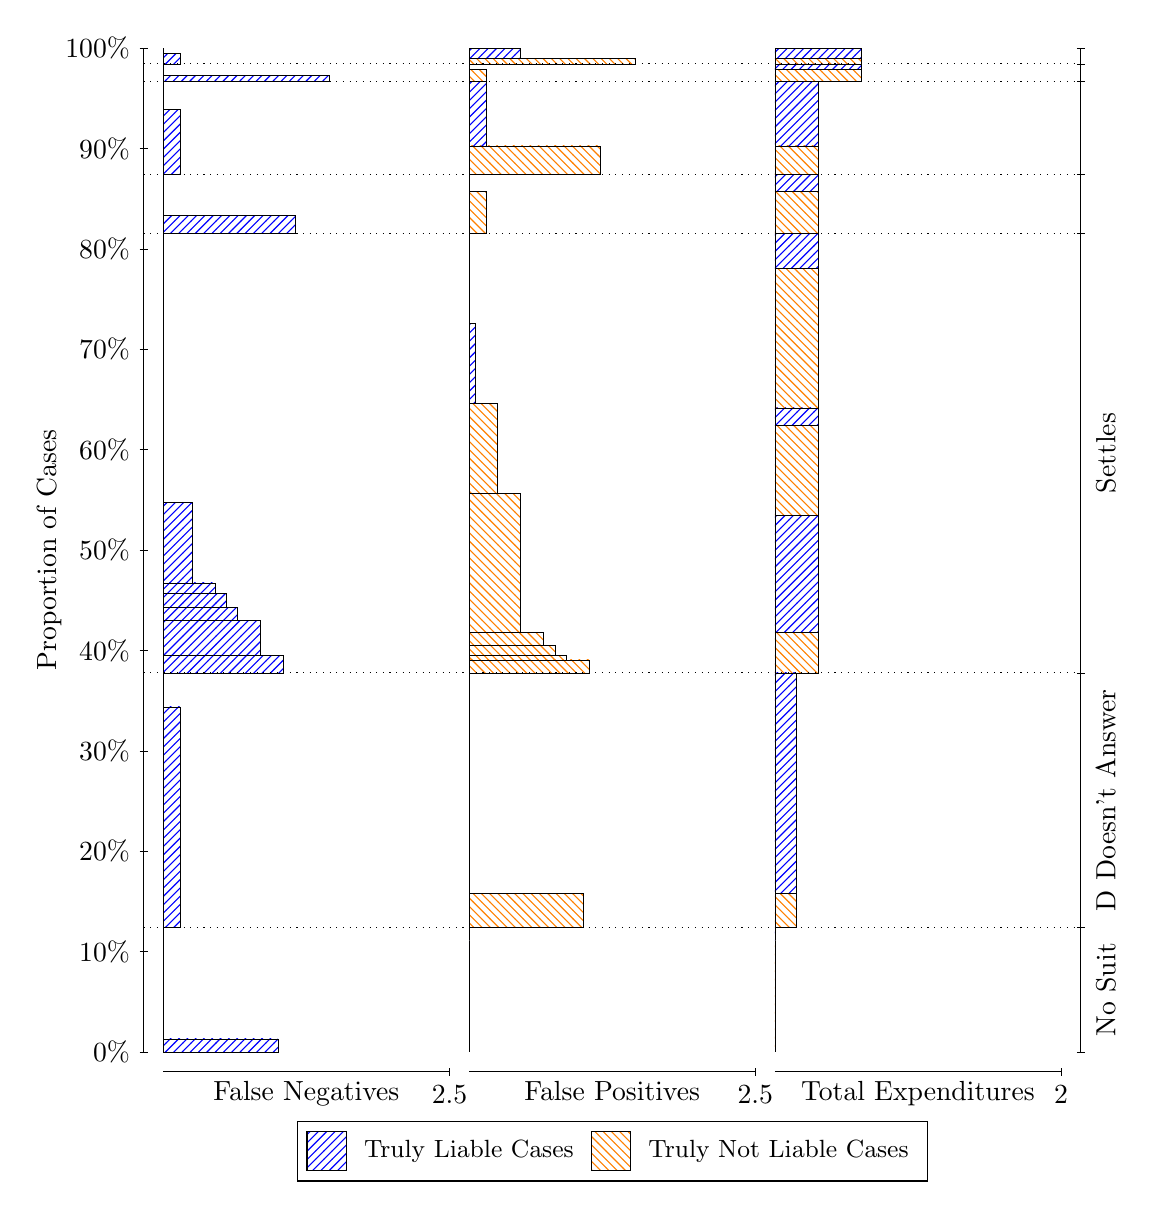
\begin{tikzpicture}
\draw[black, very thin] (1.5,1.75) -- (1.5,14.5);
\node[rotate=90, text=black, anchor=center] at (0.3, 8.125) {Proportion of Cases};
\draw[black, very thin] (1.45,1.75) -- (1.55,1.75);
\node[text=black, anchor=east] at (1.45, 1.75) {0\%};
\draw[black, very thin] (1.45,3.025) -- (1.55,3.025);
\node[text=black, anchor=east] at (1.45, 3.025) {10\%};
\draw[black, very thin] (1.45,4.3) -- (1.55,4.3);
\node[text=black, anchor=east] at (1.45, 4.3) {20\%};
\draw[black, very thin] (1.45,5.575) -- (1.55,5.575);
\node[text=black, anchor=east] at (1.45, 5.575) {30\%};
\draw[black, very thin] (1.45,6.85) -- (1.55,6.85);
\node[text=black, anchor=east] at (1.45, 6.85) {40\%};
\draw[black, very thin] (1.45,8.125) -- (1.55,8.125);
\node[text=black, anchor=east] at (1.45, 8.125) {50\%};
\draw[black, very thin] (1.45,9.4) -- (1.55,9.4);
\node[text=black, anchor=east] at (1.45, 9.4) {60\%};
\draw[black, very thin] (1.45,10.675) -- (1.55,10.675);
\node[text=black, anchor=east] at (1.45, 10.675) {70\%};
\draw[black, very thin] (1.45,11.95) -- (1.55,11.95);
\node[text=black, anchor=east] at (1.45, 11.95) {80\%};
\draw[black, very thin] (1.45,13.225) -- (1.55,13.225);
\node[text=black, anchor=east] at (1.45, 13.225) {90\%};
\draw[black, very thin] (1.45,14.5) -- (1.55,14.5);
\node[text=black, anchor=east] at (1.45, 14.5) {100\%};

\draw[black, very thin] (13.4,1.75) -- (13.4,14.5);
\draw[black, very thin] (13.35,1.75) -- (13.45,1.75);
\node[anchor=west] at (13.35, 1.75) {};
\draw[black, very thin] (13.35,3.3316) -- (13.45,3.3316);
\node[anchor=west] at (13.35, 3.3316) {};
\draw[black, very thin] (13.35,6.5639) -- (13.45,6.5639);
\node[anchor=west] at (13.35, 6.5639) {};
\draw[black, very thin] (13.35,12.149) -- (13.45,12.149);
\node[anchor=west] at (13.35, 12.149) {};
\draw[black, very thin] (13.35,12.897) -- (13.45,12.897);
\node[anchor=west] at (13.35, 12.897) {};
\draw[black, very thin] (13.35,14.077) -- (13.45,14.077);
\node[anchor=west] at (13.35, 14.077) {};
\draw[black, very thin] (13.35,14.298) -- (13.45,14.298);
\node[anchor=west] at (13.35, 14.298) {};
\draw[black, very thin] (13.35,14.5) -- (13.45,14.5);
\node[anchor=west] at (13.35, 14.5) {};

\draw[black, very thin, pattern color=blue, pattern=north east lines] (1.75,1.75) rectangle (3.2033,1.9164);
\draw[black, very thin, pattern color=orange, pattern=north west lines] (1.75,1.9164) rectangle (1.75,3.3316);
\draw[black, very thin, pattern color=blue, pattern=north east lines] (1.75,3.3316) rectangle (1.968,6.1332);
\draw[black, very thin, pattern color=orange, pattern=north west lines] (1.75,6.1332) rectangle (1.75,6.5639);
\draw[black, very thin, pattern color=blue, pattern=north east lines] (1.75,6.5639) rectangle (3.276,6.7847);
\draw[black, very thin, pattern color=blue, pattern=north east lines] (1.75,6.7847) rectangle (2.9853,7.2337);
\draw[black, very thin, pattern color=blue, pattern=north east lines] (1.75,7.2337) rectangle (2.6947,7.3945);
\draw[black, very thin, pattern color=blue, pattern=north east lines] (1.75,7.3945) rectangle (2.5493,7.5709);
\draw[black, very thin, pattern color=blue, pattern=north east lines] (1.75,7.5709) rectangle (2.404,7.7067);
\draw[black, very thin, pattern color=blue, pattern=north east lines] (1.75,7.7067) rectangle (2.1133,8.7278);
\draw[black, very thin, pattern color=orange, pattern=north west lines] (1.75,8.7278) rectangle (1.75,12.149);
\draw[black, very thin, pattern color=blue, pattern=north east lines] (1.75,12.149) rectangle (3.4213,12.371);
\draw[black, very thin, pattern color=orange, pattern=north west lines] (1.75,12.371) rectangle (1.75,12.897);
\draw[black, very thin, pattern color=blue, pattern=north east lines] (1.75,12.897) rectangle (1.968,13.717);
\draw[black, very thin, pattern color=orange, pattern=north west lines] (1.75,13.717) rectangle (1.75,14.077);
\draw[black, very thin, pattern color=blue, pattern=north east lines] (1.75,14.077) rectangle (3.8573,14.15);
\draw[black, very thin, pattern color=orange, pattern=north west lines] (1.75,14.15) rectangle (1.75,14.298);
\draw[black, very thin, pattern color=blue, pattern=north east lines] (1.75,14.298) rectangle (1.968,14.427);
\draw[black, very thin, pattern color=orange, pattern=north west lines] (1.75,14.427) rectangle (1.75,14.5);
\draw[black, very thin, pattern color=orange, pattern=north west lines] (5.6333,1.75) rectangle (5.6333,3.1652);
\draw[black, very thin, pattern color=blue, pattern=north east lines] (5.6333,3.1652) rectangle (5.6333,3.3316);
\draw[black, very thin, pattern color=orange, pattern=north west lines] (5.6333,3.3316) rectangle (7.0867,3.7623);
\draw[black, very thin, pattern color=blue, pattern=north east lines] (5.6333,3.7623) rectangle (5.6333,6.5639);
\draw[black, very thin, pattern color=orange, pattern=north west lines] (5.6333,6.5639) rectangle (7.1593,6.7299);
\draw[black, very thin, pattern color=orange, pattern=north west lines] (5.6333,6.7299) rectangle (6.8687,6.7914);
\draw[black, very thin, pattern color=orange, pattern=north west lines] (5.6333,6.7914) rectangle (6.7233,6.9133);
\draw[black, very thin, pattern color=orange, pattern=north west lines] (5.6333,6.9133) rectangle (6.578,7.0742);
\draw[black, very thin, pattern color=orange, pattern=north west lines] (5.6333,7.0742) rectangle (6.2873,8.8435);
\draw[black, very thin, pattern color=orange, pattern=north west lines] (5.6333,8.8435) rectangle (5.9967,9.9855);
\draw[black, very thin, pattern color=blue, pattern=north east lines] (5.6333,9.9855) rectangle (5.706,11.007);
\draw[black, very thin, pattern color=blue, pattern=north east lines] (5.6333,11.007) rectangle (5.6333,12.149);
\draw[black, very thin, pattern color=orange, pattern=north west lines] (5.6333,12.149) rectangle (5.8513,12.676);
\draw[black, very thin, pattern color=blue, pattern=north east lines] (5.6333,12.676) rectangle (5.6333,12.897);
\draw[black, very thin, pattern color=orange, pattern=north west lines] (5.6333,12.897) rectangle (7.3047,13.258);
\draw[black, very thin, pattern color=blue, pattern=north east lines] (5.6333,13.258) rectangle (5.8513,14.077);
\draw[black, very thin, pattern color=orange, pattern=north west lines] (5.6333,14.077) rectangle (5.8513,14.225);
\draw[black, very thin, pattern color=blue, pattern=north east lines] (5.6333,14.225) rectangle (5.6333,14.298);
\draw[black, very thin, pattern color=orange, pattern=north west lines] (5.6333,14.298) rectangle (7.7407,14.371);
\draw[black, very thin, pattern color=blue, pattern=north east lines] (5.6333,14.371) rectangle (6.2873,14.5);
\draw[black, very thin, pattern color=orange, pattern=north west lines] (9.5167,1.75) rectangle (9.5167,3.1652);
\draw[black, very thin, pattern color=blue, pattern=north east lines] (9.5167,3.1652) rectangle (9.5167,3.3316);
\draw[black, very thin, pattern color=orange, pattern=north west lines] (9.5167,3.3316) rectangle (9.7892,3.7623);
\draw[black, very thin, pattern color=blue, pattern=north east lines] (9.5167,3.7623) rectangle (9.7892,6.5639);
\draw[black, very thin, pattern color=orange, pattern=north west lines] (9.5167,6.5639) rectangle (10.062,7.0742);
\draw[black, very thin, pattern color=blue, pattern=north east lines] (9.5167,7.0742) rectangle (10.062,8.5684);
\draw[black, very thin, pattern color=orange, pattern=north west lines] (9.5167,8.5684) rectangle (10.062,9.7104);
\draw[black, very thin, pattern color=blue, pattern=north east lines] (9.5167,9.7104) rectangle (10.062,9.9311);
\draw[black, very thin, pattern color=orange, pattern=north west lines] (9.5167,9.9311) rectangle (10.062,11.7);
\draw[black, very thin, pattern color=blue, pattern=north east lines] (9.5167,11.7) rectangle (10.062,12.149);
\draw[black, very thin, pattern color=orange, pattern=north west lines] (9.5167,12.149) rectangle (10.062,12.676);
\draw[black, very thin, pattern color=blue, pattern=north east lines] (9.5167,12.676) rectangle (10.062,12.897);
\draw[black, very thin, pattern color=orange, pattern=north west lines] (9.5167,12.897) rectangle (10.062,13.258);
\draw[black, very thin, pattern color=blue, pattern=north east lines] (9.5167,13.258) rectangle (10.062,14.077);
\draw[black, very thin, pattern color=orange, pattern=north west lines] (9.5167,14.077) rectangle (10.607,14.225);
\draw[black, very thin, pattern color=blue, pattern=north east lines] (9.5167,14.225) rectangle (10.607,14.298);
\draw[black, very thin, pattern color=orange, pattern=north west lines] (9.5167,14.298) rectangle (10.607,14.371);
\draw[black, very thin, pattern color=blue, pattern=north east lines] (9.5167,14.371) rectangle (10.607,14.5);
\draw[black, dotted] (1.5,3.3316) -- (13.4,3.3316);
\draw[black, dotted] (1.5,6.5639) -- (13.4,6.5639);
\draw[black, dotted] (1.5,12.149) -- (13.4,12.149);
\draw[black, dotted] (1.5,12.897) -- (13.4,12.897);
\draw[black, dotted] (1.5,14.077) -- (13.4,14.077);
\draw[black, dotted] (1.5,14.298) -- (13.4,14.298);
\draw[black, very thin] (1.75,1.5) -- (5.3833,1.5);
\node[text=black, anchor=north] at (3.5667, 1.5) {False Negatives};
\draw[black, very thin] (5.3833,1.45) -- (5.3833,1.55);
\node[text=black, anchor=north] at (5.3833, 1.45) {2.5};

\draw[black, very thin] (5.6333,1.5) -- (9.2667,1.5);
\node[text=black, anchor=north] at (7.45, 1.5) {False Positives};
\draw[black, very thin] (9.2667,1.45) -- (9.2667,1.55);
\node[text=black, anchor=north] at (9.2667, 1.45) {2.5};

\draw[black, very thin] (9.5167,1.5) -- (13.15,1.5);
\node[text=black, anchor=north] at (11.333, 1.5) {Total Expenditures};
\draw[black, very thin] (13.15,1.45) -- (13.15,1.55);
\node[text=black, anchor=north] at (13.15, 1.45) {2};

\node[text=black, centered, rotate=90] at (13.72, 2.5408) {No Suit};
\node[text=black, centered, rotate=90] at (13.72, 4.9478) {D Doesn't Answer};
\node[text=black, centered, rotate=90] at (13.72, 9.3567) {Settles};





\draw (7.449999999999999,1.5) node[draw=none] (baseCoordinate) {};
\begin{scope}[align=center]
        \matrix[scale=0.5, draw=black, below=0.5cm of baseCoordinate, nodes={draw}, column sep=0.1cm]{
            \node[rectangle, draw, minimum width=0.5cm, minimum height=0.5cm, pattern color=blue, pattern=north east lines] {}; &
            \node[draw=none, font=\small, text=black] (B) {Truly Liable Cases}; &
            \node[rectangle, draw, minimum width=0.5cm, minimum height=0.5cm, pattern color=orange, pattern=north west lines] {}; &
            \node[draw=none, font=\small, text=black] (B) {Truly Not Liable Cases}; \\
            };
\end{scope}

\end{tikzpicture}
\end{document}